\documentclass[12pt,]{article}
\usepackage{lmodern}
\usepackage{amssymb,amsmath}
\usepackage{ifxetex,ifluatex}
\usepackage{fixltx2e} % provides \textsubscript
\ifnum 0\ifxetex 1\fi\ifluatex 1\fi=0 % if pdftex
  \usepackage[T1]{fontenc}
  \usepackage[utf8]{inputenc}
\else % if luatex or xelatex
  \ifxetex
    \usepackage{mathspec}
  \else
    \usepackage{fontspec}
  \fi
  \defaultfontfeatures{Ligatures=TeX,Scale=MatchLowercase}
\fi
% use upquote if available, for straight quotes in verbatim environments
\IfFileExists{upquote.sty}{\usepackage{upquote}}{}
% use microtype if available
\IfFileExists{microtype.sty}{%
\usepackage{microtype}
\UseMicrotypeSet[protrusion]{basicmath} % disable protrusion for tt fonts
}{}
\usepackage[left=1in, right=1in, top=1in, bottom=1in, headheight=12pt, letterpaper]{geometry}
\usepackage{hyperref}
\hypersetup{unicode=true,
            pdftitle={A simulation-based approach for quantifying and partitioning uncertainty to improve forecasts of dynamic processes},
            pdfauthor={Andrew T. Tredennick\^{}\{1\}, Peter B. Adler\^{}1, and others\^{}\{2\}},
            pdfborder={0 0 0},
            breaklinks=true}
\urlstyle{same}  % don't use monospace font for urls
\usepackage{graphicx,grffile}
\makeatletter
\def\maxwidth{\ifdim\Gin@nat@width>\linewidth\linewidth\else\Gin@nat@width\fi}
\def\maxheight{\ifdim\Gin@nat@height>\textheight\textheight\else\Gin@nat@height\fi}
\makeatother
% Scale images if necessary, so that they will not overflow the page
% margins by default, and it is still possible to overwrite the defaults
% using explicit options in \includegraphics[width, height, ...]{}
\setkeys{Gin}{width=\maxwidth,height=\maxheight,keepaspectratio}
\IfFileExists{parskip.sty}{%
\usepackage{parskip}
}{% else
\setlength{\parindent}{0pt}
\setlength{\parskip}{6pt plus 2pt minus 1pt}
}
\setlength{\emergencystretch}{3em}  % prevent overfull lines
\providecommand{\tightlist}{%
  \setlength{\itemsep}{0pt}\setlength{\parskip}{0pt}}
\setcounter{secnumdepth}{0}
% Redefines (sub)paragraphs to behave more like sections
\ifx\paragraph\undefined\else
\let\oldparagraph\paragraph
\renewcommand{\paragraph}[1]{\oldparagraph{#1}\mbox{}}
\fi
\ifx\subparagraph\undefined\else
\let\oldsubparagraph\subparagraph
\renewcommand{\subparagraph}[1]{\oldsubparagraph{#1}\mbox{}}
\fi

%%% Use protect on footnotes to avoid problems with footnotes in titles
\let\rmarkdownfootnote\footnote%
\def\footnote{\protect\rmarkdownfootnote}

%%% Change title format to be more compact
\usepackage{titling}

% Create subtitle command for use in maketitle
\newcommand{\subtitle}[1]{
  \posttitle{
    \begin{center}\large#1\end{center}
    }
}

\setlength{\droptitle}{-2em}
  \title{A simulation-based approach for quantifying and partitioning uncertainty
to improve forecasts of dynamic processes}
  \pretitle{\vspace{\droptitle}\centering\huge}
  \posttitle{\par}
  \author{Andrew T. Tredennick\(^{1}\), Peter B. Adler\(^1\), and others\(^{2}\)}
  \preauthor{\centering\large\emph}
  \postauthor{\par}
  \date{}
  \predate{}\postdate{}

\usepackage[textsize=tiny,textwidth=2.1cm]{todonotes}
\usepackage{mathptmx}
\usepackage{upgreek}
\usepackage{bm}
\usepackage{setspace}
\usepackage{booktabs}
\doublespacing
\usepackage{lineno}
\linenumbers
\usepackage{floatrow}
\newcounter{box}
\newcommand{\boxnumber}{\addtocounter{box}{1} \thebox \thinspace}
\floatstyle{boxed}
\newfloat{Box}{tbph}{box}
\floatsetup[table]{capposition=top}

\begin{document}
\maketitle

\newcommand{\smalltodo}[2][]
    {\todo[caption={#2}, #1]
    {\begin{spacing}{0.5}#2\end{spacing}}}\setlength{\abovedisplayskip}{0pt}\raggedright\setlength{\parindent}{36pt}

\noindent{}\(^1\) Department of Wildland Resources and the Ecology
Center, Utah State University, Logan, UT, United States

\noindent{}\(^2\) Department of somewhere

\hypertarget{abstract}{%
\section{Abstract}\label{abstract}}

Making informed decisions in the face of rapid environmental change
requires forecasts from models of ecological processes. However,
forecasts from ecological models are often associated with high degrees
of uncertainty, making it difficult for such forecasts to inform
decision-making processes. To make progress toward the goal of reliable
and informative ecological forecasts, we need to know from where
forecast uncertainty arises. Such knowledge can guide investment in
future research that will most improve forecast skill. There is a rich
history of analytical expressions that partition the variance of future
dynamics, but these expressions suffer from necessary assumptions such
as linear dynamics and small-variance approximations that exclude
interactions. Similarly, the earth systems modeling community has
developed methods for paritioning uncertainty of model projections, but
these operate at a different modeling grain than most of ecology.
Building on these approaches, we develop a simulation-based approach for
quantifying and partitioning forecast uncertainty from Bayesian
state-space models that overcomes the limitations of previous analytical
approaches. Our approach is similar to an Analysis of Variance, where
the total variance of a forecast is paritioned among its constituent
parts, namely initial conditions uncertainty, parameter uncertainty,
driver uncertainty, process error, and their interactions. We apply the
approach to near-term forecasts of the Yellowstone bison population and
measles in China, demonstrating the broad utility of our approach. We
also provide functions written in the statistical programming language
R, which will allow others using Bayesian state-space models to employ
our approach in their own research.

\emph{Keywords: Bayesian state-space model, forecast, Markov chain Monte
Carlo, measles, prediction, population model, uncertainty, Yellowstone
bison}

\hypertarget{introduction}{%
\section{Introduction}\label{introduction}}

A fundamental challenge facing society is to predict the ecological
impacts of global environmental changes such as nitrogen deposition,
climate change, and habitat fragmentation. Each of these global change
drivers have now exceeded their historical ranges of variability
(Steffen et al. 2015), ushering in a no-analog era in which the past
cannot predict the future. We can, however, look to the past to
parameterize models that allow us to forecast the future states of
ecological systems (Clark et al. 2001, Dietze et al. 2018). Ecologists
are in an excellent position to meet this forecasting challenge because
we have spent decades gaining understanding of the processes that
regulate populations, communities, and ecosystems. However, we lack a
systematic understanding of the current limits to ecological forecasts.
As a result, we do not know how to allocate research effort to improve
our forecasts.

Making poor forecasts is inevitable as ecology matures into a more
predictive science. The key is to learn from our failures so that
forecasts become more accurate over time. The success of meteorological
forecasting tells us that basic research on the causes of forecast
uncertainty is an essential component of this learning process (Bauer et
al. 2015).

Various approaches have been used to characterize and partition forecast
uncertainty (Sobol' 1993, Cariboni et al. 2007). For example, consider a
dynamic model designed to predict some state \emph{y} in the future
(\(y_{t+1}\)) based on the current state (\(y_{t}\)), an environmental
driver(s) (\(x\)), parameters (\(\theta\)), and process error
(\(\epsilon\)). We can then write a general form of the model as:

\begin{align}
y_{t+1} = f(y_t, x_t|\theta) + \epsilon_{t+1},
\end{align}

\noindent{}which states that \(y\) at time \(t+1\) is a function of
\(y\) and \(x\) at time \(t\) conditional on the model parameters
(\(\theta\)) plus process error (\(\epsilon\)). Ignoring covariance
among factors and assuming linear dynamics, Dietze (2017), following
Sobol' (1993) and Cariboni et al. (2007), suggests that forecast
variance (\(Var[y_{t+1}]\)) is approximately:

\begin{align}
Var[y_{t+1}] \approx \underbrace{\left(\frac{\delta f}{\delta y} \right)^2}_{\text{stability}} 
               \underbrace{\vphantom{ \left(\frac{\delta f}{\delta y} \right)^2 } Var[y_t]}_{\text{IC uncert.}} +
               \underbrace{\vphantom{ \left(\frac{\delta f}{\delta y} \right)^2 }\left(\frac{\delta f}{\delta x} \right)^2}_{\text{driver sens.}} 
               \underbrace{\vphantom{ \left(\frac{\delta f}{\delta y} \right)^2 } Var[x_t]}_{\text{driver uncert.}} +
               \underbrace{\vphantom{ \left(\frac{\delta f}{\delta y} \right)^2 }\left(\frac{\delta f}{\delta \theta} \right)^2}_{\text{param sens.}}
               \underbrace{\vphantom{ \left(\frac{\delta f}{\delta y} \right)^2 } Var[\theta]}_{\text{param. uncert.}} +
               \underbrace{\vphantom{ \left(\frac{\delta f}{\delta y} \right)^2 } Var[\epsilon_{t+1}]}_{\text{process error}},
\end{align}

\noindent{}where each additive term follows a pattern of
\emph{sensitivity} times \emph{variance} and ``IC uncert.'' refers to
``\emph{I}nitial \emph{C}onditions uncertainty.'' The variance
attributable to any particular factor is a function of how sensitive the
model is to the factor and the variance of that factor. For example, the
atmosphere is a chaotic system, meaning its dynamics are internally
unstable and sensitive to initial conditions uncertainty. This is why
billions of dollars are spent each year to measure meterological
variables -- meterologists learned that the key to reducing forecast
error \((Var[y_{t+1}])\) was to reduce the uncertainty of initial
conditions (\(Var[y_t]\)). In contrast, ecologists are attempting to
make actionable forecasts with little knowledge of which term in Eq. 2
dominates forecast error. Knowing which term dominates forecast error in
different ecological settings will advance our fundamental understanding
of the natural world and immediately impact practical efforts to
monitor, model, and predict ecological dynamics.

While having an analytical expression such as Eq. 2 is satisfying,
arriving at the expression involves strict assumptions. First, Eq. 2
only holds when the underlying dynamics are linear, which may not be the
case for many populations and models. Second, Eq. 2 only includes
additive effects of each factor because the Taylor series decomposition
requires small-variance approximations that eliminate interactions. But,
interactions among the factors are probably commone. For example, in a
simple simulation of an AR(1) process, we show that initial conditions
uncertainty and parameter error interact to generate the full spread of
forecast variance (Figure 1). Therefore, progress in quantifying and
partioning forecast uncertainty requires a more flexible approach than
that provided by Eq. 2.

\begin{figure}
\centering
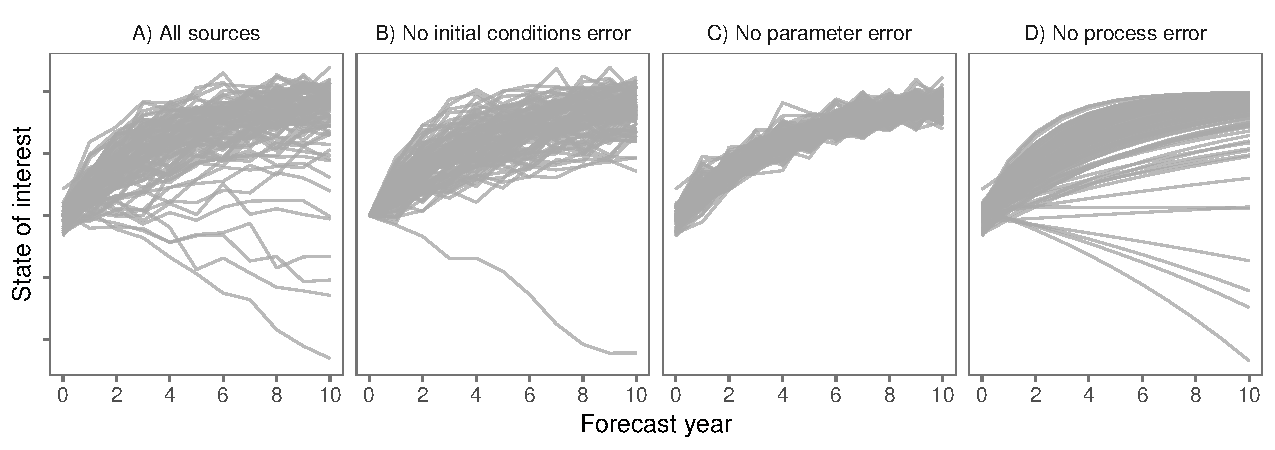
\includegraphics{../figures/forecast_uncertainty_example.pdf}
\caption{Example of forecast uncertainty with different sources of error
set to zero. Each line represents one realization, out of 200, from an
order-one autoregressive model (AR1 process). Contrary to the analytical
expression (Eq. 2), initial conditions uncertainty and parameter
uncertainty clearly interact. The spread of lines in (A) is not wholly
because of initial conditions uncertainty (B) or parameter uncertainty
(C), it is their combined influence that causes the spread of
realizations in (A). At least in this example, process error (D) does
appear to be independent, but we used a small value of process error to
highlight other interactions. Source code:
\texttt{generate\_forecast\_fxns.R}.}
\end{figure}

\hypertarget{a-brief-history-of-quantifying-and-partitioning-forecast-uncertainty}{%
\section{A Brief History of Quantifying and Partitioning Forecast
Uncertainty}\label{a-brief-history-of-quantifying-and-partitioning-forecast-uncertainty}}

\hypertarget{error-propagation}{%
\subsection{Error propagation}\label{error-propagation}}

Methods for quantifying and partitioning forecast uncertainty all share
common roots in statistical error propagation. Error propagation is
concerned with translating the effects of variable (or parameter)
uncertainty into the uncertainty of a function based those variables.
That is, for the output \emph{q} of some function
\(q = f(x_1,x_2,\dots,x_n)\), we are interested in the variance of
\emph{q} given the variance of input variables (\textbf{x}). It is this
generic model formulation that leads to the canonical expression of
error propagation

\begin{align}
\sigma^2_q &= \left( \frac{\delta q}{\delta x_1} \sigma_{x_1} \right)^2 + \left( \frac{\delta q}{\delta x_2} \sigma_{x_2} \right)^2 + \cdots + \left( \frac{\delta q}{\delta x_n} \sigma_{x_n} \right)^2 \\
&= \sum^n_{i=1}\left( \frac{\delta q}{\delta x_i} \sigma_{x_i} \right)^2.
\end{align}

\noindent{}This expression states that the variance of the output of
function \(q\) (\(\sigma^2_q\)) is equal to the sum of squares of the
input variables weighted by the sensitivity of the output variable to
each input variable, quantified as the partial derivative.

\hypertarget{weather-forecasting}{%
\subsection{Weather forecasting}\label{weather-forecasting}}

Chaos.

\hypertarget{earth-system-models}{%
\subsection{Earth system models}\label{earth-system-models}}

Carbon.

\hypertarget{dynamical-models}{%
\subsection{Dynamical models}\label{dynamical-models}}

Lotka-Volterra.

\hypertarget{a-simulation-based-approach-for-partitioning-forecast-uncertainty}{%
\section{A Simulation-Based Approach for Partitioning Forecast
Uncertainty}\label{a-simulation-based-approach-for-partitioning-forecast-uncertainty}}

Analytical expressions of forecast uncertainty must rely on simplifying
assumptions. Two important assumptions are (1) that different sources of
uncertainty do not interact and (2) that the system of equations is
linear. These analytical expressions are important for guiding our
intuition, but these strict assumptions limit our ability to partition
forecast uncertainty in practice. Thus, we present a simulation approach
that is entirely model-based and requires no assumptions, other than
those embedded in the model itself. We are building on the ideas put
forth by Dietze (2017), who suggested a simulation approach for
quantifying the terms in Eq. 2. Here we test the general idea using
simulated data and extend the approach to consider interactions among
sources of uncertainty.

As a starting point, consider a generic Bayesian state-space model

\begin{equation}
\begin{aligned}[b]
\textbf{Data Model:} \quad y_t &\sim \left[y_t \;|\; z_t, \sigma^2_{\text{o}}\right], &t = 1,\dots,T, \\ 
\textbf{Process Models:} \quad z_t &\sim \left[z_t \;|\; \mu_t, \sigma^2_{\text{p}}\right],  \\ 
\mu_t &= g \left(z_{t-1},\textbf{x}'_t, \bm{\uptheta} \right), &t = 2,\dots,T, \\ 
\textbf{Parameter Models:} \quad \bm{\upphi} &\sim \left[\bm{\uptheta},\sigma^2_{\text{p}},\sigma^2_{\text{o}},z_{t=1} \right],
\end{aligned}
\end{equation}

\noindent{}where \(y_t\) is the observed state at time \emph{t}, \(z_t\)
is the latent state at time \emph{t}, \(\mu_t\) is the determinstic
prediction of \emph{z} at time \emph{t} from the process model \emph{g},
which is a function of \emph{z} at time \emph{t-1}, a vector of
covariates (\textbf{x}) at time \emph{t}, and a set of unknown
parameters, \(\bm{\uptheta}\). \(\sigma^2_{\text{o}}\) is observation
error and \(\sigma^2_{\text{p}}\) is process error. The notation
\(\left[a \;|\; b, c\right]\) reads, ``the probability of \emph{a} given
\emph{b} and \emph{c}'' (Gelfand and Smith 1990), and \(\bm{\upphi}\)
refers to the prior probability distributions for all unknown parameters
and the initial conditions for the latent state, \(z_{t=1}\).

For our purposes, we are interested in the probability distributions of
the true state \textbf{z} at future points in time, conditional on
previous observations (\textbf{y}). This is referred to as the forecast
distribution or the predictive process distribution (Hobbs and Hooten
2015 pp. 199--200), which, for one time step ahead of the final
observation (\(T+1\)), is defined as

\begin{equation}
\begin{gathered}
\left[z_{T+1} | y_1,\dots,y_T \right] = \int \int \dots \int \left[z_{T+1} | z_T, \textbf{x}_T, \bm{\uptheta}, \sigma^2_{\text{p}} \right] \\ \times \left[z_1,\dots,z_{T+1},\bm{\uptheta}, \sigma^2_{\text{p}} | y_1,\dots,y_T \right] d\bm{\uptheta} d\sigma^2_{\text{p}} dz_1 \dots dz_T.
\end{gathered}
\end{equation}

The model in Eq. 5 can be fit using Markov chain Monte carlo (MCMC)
algorithms, which makes calculating the forecast distribution a
relatively simple task. To obtain
\(\left[z_{T+1} | y_1,\dots,y_T \right]\), we can change the indexing of
\emph{t} in Eq. 5 to \(t = 2,\dots,T+1\) and then sample
\(z_{T+1}^{(k)}\) from
\(\left[z_{T+1} | g(z_T^{(k)}, \textbf{x}_{T+1}^{(j(k))}, \bm{\uptheta}^{(k)}), \sigma^{2(k)}_{\text{p}} \right]\)
given the current values for \(\bm{\uptheta}^{(k)}\) and \(z_{T}^{(k)}\)
on each \(k = 1,\dots,K\) iteration of the MCMC algorithm (Hobbs and
Hooten 2015, Williams et al. 2018). Note that we index the external
covariate vector \textbf{x} using \emph{j} and \emph{k}, where
\emph{j(k)} is realization \emph{j} of the covariate vector \textbf{x}
associated with MCMC sample \emph{k}. In some cases, the external
covariate will have only one value, in which case all \emph{K} MCMC
samples will share the same \textbf{x}. In other cases, their may be a
distribution of external covariate values associated with uncertainty
from the forecast of \textbf{x}, resulting in \emph{n} values for each
\(x_{T+1}\). When \(n < K\), which we anticipate it often will be, then
\textbf{x} can be sampled with replacement and a value can be assigned
to each MCMC sample. Making forecasts further into the future than
\(T+1\) requires extending \(T+1\) to \(T+2,\dots,T+q\) and iteratively
sampling
\(\left[z_{T+q} | g(z_{T+q-1}^{(k)}, \textbf{x}_{T+q}^{(j(k))},\bm{\uptheta}^{(k)}), \sigma^{2(k)}_{\text{p}} \right]\)
(Hobbs and Hooten 2015).

The forecast distribution (Eq. 6) has all of the quantities that
contribute to forecast uncertainty by incorporating their uncertainty
explicitly across the \emph{K} MCMC iterations. For example, initial
conditions uncertainty is incorporated because \(z_{T+1}^{(k)}\) is a
function of \(z_{T}^{(k)}\), resulting in a total of \emph{K} point
forecasts for \emph{z} that comprise the posterior distribution of
\emph{z} at each time \emph{t}. If we wish to ignore initial conditions
uncertainty (I.C. uncertainty), we can make all \emph{K} point forecasts
starting from the mean of \(z_{T}\)

\begin{equation}
z_{T}^{(*)} = E(z_{T} | y_1,\dots,y_T) \approx \frac{\sum^K_{k=1} z_{T}^{(k)}}{K},
\end{equation}

\noindent{}which we call \(z^{(*)}_T\) (as opposed to \(z^{(k)}_T\)),
while retaining the uncertainty around all other parameters. Our
iterative sampling to obtain the forecast distribution then becomes a
conditional statement,

\begin{equation}
\begin{aligned}[b]
z_{T+q} &\sim \left[z_{T+q} | g(z_{T+q-1}^{(k)}, \textbf{x}_T^{(j(k))}, \bm{\uptheta}^{(k)}), \sigma^{2(k)}_{\text{p}} \right], &q>1 \\
z_{T+q} &\sim \left[z_{T+q} | g(z_{T}^{(*)}, \textbf{x}_T^{(j(k))}, \bm{\uptheta}^{(k)}), \sigma^{2(k)}_{\text{p}} \right], &q=1.
\end{aligned}
\end{equation}

\noindent{}We can extend the basic idea of setting subsets of parameters
and states to their posterior means (or medians, depending on the
distribution) to make partitioned forecasts where only prescribed
sources of uncertainty contribute to forecast uncertainty (Table 1).

\renewcommand{\arraystretch}{1.6}\begin{table}[ptb]
\centering 
\begin{tabular}{l l l l l}
\toprule
\textbf{Source of Uncertainty} & \textbf{Notation} && \textbf{Sampling Equation} & \\
\midrule 
I.C. Uncertainty & $V^{(I)} = V^{(I,\overline{PA},\overline{D},\overline{PS})}$ &&  $\left[z_{T+q} \; | \; g(z_{T+q-1}^{(k)}, \textbf{x}^{(*)}_T, \bm{\uptheta}^{(*)}), 0 \right]$ & \\
\addlinespace[0.3cm]
Parameter Uncertainty & $V^{(PA)} = V^{(\overline{I},PA,\overline{D},\overline{PS})}$ && $\left[z_{T+q} \; | \; g(z_{T+q-1}^{(k)}, \textbf{x}^{(*)}_T, \bm{\uptheta}^{(k)}), 0 \right]$, & $q>1$ \\
 &&& $\left[z_{T+q} \; | \; g(z_{T}^{(*)}, \textbf{x}^{(*)}_T, \bm{\uptheta}^{(k)}), 0 \right]$, & $q=1$ \\
  \addlinespace[0.3cm]
Driver Uncertainty & $V^{(D)} = V^{(\overline{I},\overline{PA},D,\overline{PS})}$ && $\left[z_{T+q} \; | \; g(z_{T+q-1}^{(k)}, \textbf{x}^{(j(k))}_T, \bm{\uptheta}^{(*)}), 0 \right]$, & $q>1$ \\
 &&& $\left[z_{T+q} \; | \; g(z_{T}^{(*)}, \textbf{x}^{(j(k))}_T, \bm{\uptheta}^{(*)}), 0 \right]$, & $q=1$ \\
 \addlinespace[0.3cm]
Process Uncertainty & $V^{(PS)}=V^{(\overline{I},\overline{PA},\overline{D},PS)}$ && $\left[z_{T+q} \; | \; g(z_{T+q-1}^{(k)}, \textbf{x}^{(*)}_T, \bm{\uptheta}^{(*)}), \sigma^{2(k)}_{\text{p}} \right]$, & $q>1$ \\
 &&& $\left[z_{T+q} \; | \; g(z_{T}^{(*)}, \textbf{x}^{(*)}_T, \bm{\uptheta}^{(*)}), \sigma^{2(k)}_{\text{p}} \right]$, & $q=1$ \\
\bottomrule 
\end{tabular}
\caption{Sampling equations for generating forecasts at times $T+q$ (where $T$ is the time of the last observation) with only certain sources of uncertainty present.}   
\label{tab:sampling_formulas}
\end{table}\renewcommand{\arraystretch}{1.0}

It is important to note that although our discussion has centered on
obtaining forecast distributions within the MCMC algorithm used to fit
the model, it is only feasible to do this for the full forecast
distribution (Eq. 6). In all other cases, where states or parameters
must be averaged over the \emph{K} MCMC iterations, forecast simulations
must be done \emph{post hoc} using saved MCMC samples (Box 1). In other
words, estimating \(z_1,z_2,\dots,z_T\) is done within the MCMC fitting
algorithm, while estimating \(z_{T+1},z_{T+2},\dots,z_{T+q}\) is done
after fitting the model, but with the full MCMC output.

With these basics in mind, we now develop our approach for partitioning
and quantifying uncertainty, which is similar to an Analysis of Variance
(ANOVA). Let the variance of the forecast distribution at time \(T+q\)
be \(V^{(X)}_{T+q}\), where \(X=F\) (full forecast distribution), \(I\)
(initial conditions uncertainty only), \(PA\) (parameter uncertainty
only), \(D\) (driver uncertainty), or \(PS\) (process uncertainty only)
(Table 1). \(V_{T+q}^{(I)}\), \(V_{T+q}^{(PA)}\), \(V_{T+q}^{(D)}\), and
\(V_{T+q}^{(PS)}\) are the main effects of each factor on the forecast
distribution such that

\begin{equation}
\begin{aligned}[b]
V_{T+q}^{(F)} = \ &V_{T+q}^{(I)} + V_{T+q}^{(PA)} + V_{T+q}^{(D)} + V_{T+q}^{(PS)} \\
&+ \epsilon_{T+q}^{(I,PA)} + \epsilon_{T+q}^{(I,D)} + \epsilon_{T+q}^{(I,PS)} + \epsilon_{T+q}^{(PA,PS)} + \epsilon_{T+q}^{(PA,D)} + \epsilon_{T+q}^{(D,PS)} \\
&+ \epsilon_{T+q}^{(I,PA,D)} + \epsilon_{T+q}^{(I,PA,PS)} + \epsilon_{T+q}^{(I,D,PS)} + \epsilon_{T+q}^{(PA,D,PS)} \\
&+ \epsilon_{T+q}^{(I,PA,D,PS)},
\end{aligned}
\end{equation}

\noindent{}where the notation \(\epsilon_{T+q}^{(X,Y)}\) represents the
remaining interactive effect of \(X\) and \(Y\) on \(V_{T+q}^{(F)}\)
after accounting for their main effects. For example, if the full
forecast variance is a function of only initial conditions uncertainty
\emph{I} and parameter uncertainty \emph{PA}, then

\begin{equation}
V^{(F)}_{T+q} = V^{(I)}_{T+q} + V^{(PA)}_{T+q} + \epsilon_{T+q}^{(I,PA)},
\end{equation}

\noindent{}which rearranges to

\begin{equation}
\epsilon_{T+q}^{(I,PA)} = V^{(F)}_{T+q} - \left[ V^{(I)}_{T+q} + V^{(PA)}_{T+q} \right].
\end{equation}

\noindent{}We show an example of applying Eqs. 10-11 in a hypothetical
situation where forecast uncertainty is determined by initial conditions
uncertainty and parameter uncertainty alone (Figure 2). The necessary
terms for partitioning forecast variance can be obtained by calculating
the variance of the partitioned forecast distributions (equations in
Table 1 and combinations thereof). To take this one step further, and to
reiterate the core idea, let \(V(F)\) be a function of initial
conditions uncertainty \emph{I}, parameter uncertainty \emph{PA}, and
driver uncertainty \emph{D}. We can then write the equation for forecast
uncertainty and the derived interaction effects as

\begin{align}
V^{(F)}_{T+q} &= V^{(I)}_{T+q} + V^{(PA)}_{T+q} + V^{(D)}_{T+q} + \epsilon^{(I,PA)}_{T+q} + \epsilon^{(I,D)}_{T+q} + \epsilon^{(D,PA)}_{T+q} + \epsilon^{(I,PA,D)}_{T+q}, \qquad \text{where} \\
\epsilon^{(I,PA)}_{T+q} &= V^{(F)}_{T+q} - 
\end{align}

\begin{figure}
\centering
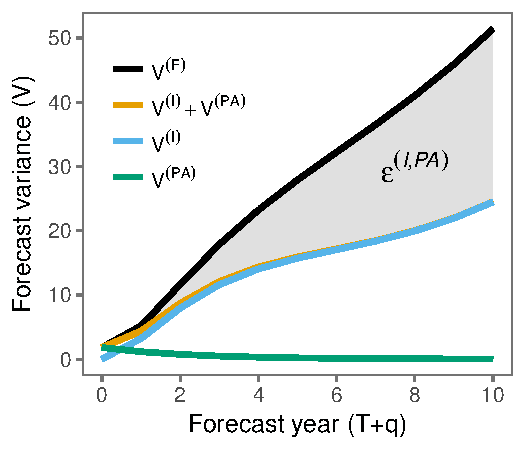
\includegraphics[width=\textwidth,height=3in]{../figures/example_interaction_effect.pdf}
\caption{Graphical example of partitioning forecast uncertainty into
main effects (\(V\)) and interaction effects (\(\epsilon\)). The grey
shaded area shows the interaction effect (\(\epsilon^{(I,PA)}\)) that
must be accounted for to fully partition forecast uncertainty between
initial conditions uncertainty (\(V^{(I)}\)) and parameter uncertainty
(\(V^{(PA)}\)). Source code: \texttt{generate\_forecast\_fxns.R}.}
\end{figure}

\begin{Box}
  \renewcommand{\arraystretch}{1.04}
  \caption{}
  \textbf{Box 1.} Pseudocode for quantifying and partitioning forecast uncertainty from a Bayesian state-space model. 
  \vspace{1em}
  \begin{enumerate}
    \item Fit a Bayesian state-space model (i.e., Eq. 5) with data $y_1,\dots,y_T$ and save the MCMC samples.
    \item Forecast $z_{T+q}^{(k)}$ for all $k = 1,\dots,K$ MCMC samples to generate the full forecast distribution following Eq. 6 (this can be done within the MCMC algorithm or \emph{post hoc} with saved MCMC samples).
    \item Forecast $z_{T+q}^{(k)}$ for all $k = 1,\dots,K$ MCMC samples to generate the partitioned forecast distributions for each source of uncertainty, averaging quantities over the $K$ MCMC samples as necessary (equations in Table 1 and combinations thereof).
    \item For each forecast time $q$, calculate the variance of each forecast distribution from steps 2-3.
    \item Partition forecast variance using Eq. X.
  \end{enumerate}
  \renewcommand{\arraystretch}{1.0}
\end{Box}

\hypertarget{application-yellowstone-bison-population}{%
\section{Application: Yellowstone Bison
Population}\label{application-yellowstone-bison-population}}

\hypertarget{application-measles-in-china}{%
\section{Application: Measles in
China}\label{application-measles-in-china}}

\hypertarget{discussion}{%
\section{Discussion}\label{discussion}}

\hypertarget{acknowledgements}{%
\section{Acknowledgements}\label{acknowledgements}}

This research was funded by National Science Foundation grants
DEB-1353078 (awarded to PBA) and DEB-1353039 (awarded to Stephen P.
Ellner and Giles Hooker).

\setlength{\parindent}{0pt}

\hypertarget{references}{%
\section{References}\label{references}}

\hypertarget{refs}{}
\leavevmode\hypertarget{ref-Bauer2015}{}%
Bauer, P., A. Thorpe, and G. Brunet. 2015. The quiet revolution of
numerical weather prediction. Nature 525:47--55.

\leavevmode\hypertarget{ref-Cariboni2007}{}%
Cariboni, J., D. Gatelli, R. Liska, and A. Saltelli. 2007. The role of
sensitivity analysis in ecological modelling. Ecological Modelling
203:167--182.

\leavevmode\hypertarget{ref-Clark2001}{}%
Clark, J. S., S. R. Carpenter, M. Barber, S. Collins, A. Dobson, J. A.
Foley, D. M. Lodge, M. Pascual, R. Pielke, W. Pizer, C. Pringle, W. V.
Reid, K. A. Rose, O. Sala, W. H. Schlesinger, D. H. Wall, and D. Wear.
2001. Ecological forecasts: an emerging imperative. Science
293:657--660.

\leavevmode\hypertarget{ref-Dietze2017a}{}%
Dietze, M. C. 2017. Prediction in ecology: A first-principles framework.
Ecological Applications 27:2048--2060.

\leavevmode\hypertarget{ref-Dietze2018}{}%
Dietze, M. C., A. Fox, L. M. Beck-Johnson, J. L. Betancourt, M. B.
Hooten, C. S. Jarnevich, T. H. Keitt, M. A. Kenney, C. M. Laney, L. G.
Larsen, H. W. Loescher, C. K. Lunch, B. C. Pijanowski, J. T. Randerson,
E. K. Read, A. T. Tredennick, R. Vargas, K. C. Weathers, and E. P.
White. 2018. Iterative near-term ecological forecasting: Needs,
opportunities, and challenges. Proceedings of the National Academy of
Sciences 115:1424--1432.

\leavevmode\hypertarget{ref-Gelfand1990}{}%
Gelfand, A. E., and A. F. Smith. 1990. Sampling-based approaches to
calculating marginal densities. Journal of the American Statistical
Association 85:398--409.

\leavevmode\hypertarget{ref-Hobbs2015}{}%
Hobbs, N. T., and M. B. Hooten. 2015. Bayesian Models: A Statistical
Primer for Ecologists. Princeton University Press, Princeton.

\leavevmode\hypertarget{ref-Sobol1993}{}%
Sobol', I. 1993. Sensitivity Estimates for Nonlinear Mathematical
Models.

\leavevmode\hypertarget{ref-Steffen2015}{}%
Steffen, W., K. Richardson, J. Rockström, S. Cornell, I. Fetzer, E.
Bennett, R. Biggs, and S. Carpenter. 2015. Planetary boundaries: Guiding
human development on a changing planet. Science 348:1217.

\leavevmode\hypertarget{ref-Williams2018}{}%
Williams, P. J., M. B. Hooten, J. N. Womble, G. G. Esslinger, and M. R.
Bower. 2018. Monitoring dynamic spatio-temporal ecological processes
optimally. Ecology 99:524--535.


\end{document}
